\documentclass[addpoints]{exam}

% \pagestyle{empty}                       %no page numbers
% \thispagestyle{empty}                   %removes first page number
% \setlength{\parindent}{0in}               %no paragraph indents

\usepackage{fullpage}
\usepackage[tmargin = 0.5in, bmargin = 1in, hmargin = 1in]{geometry}     %1-inch margins
\geometry{letterpaper}                  
\usepackage{graphicx}
\usepackage{amssymb}

% Default packages
\usepackage{latexsym}
\usepackage{amsfonts}
\usepackage{amsmath}
\usepackage{amsthm}
\usepackage{hyperref}
\usepackage{multicol}
\usepackage{multirow}
\usepackage{enumerate}
\usepackage{enumitem}


%% Definitions
\def\va{\mathbf{a}}
\def\vb{\mathbf{b}}
\def\vc{\mathbf{c}}
\def\vx{\mathbf{x}}
\def\vzero{\mathbf{0}}



\def\vi{\mathbf{i}}
\def\vj{\mathbf{j}}
\def\vk{\mathbf{k}}
\def\vr{\mathbf{r}}
\def\vu{\mathbf{u}}
\def\vv{\mathbf{v}}
\def\pageturn{\vfill
\begin{flushright}
	\begin{small}
		Continued $\rightarrow$
	\end{small}
\end{flushright}
\newpage}

\pagestyle{headandfoot}
\runningheadrule
\firstpageheader{\textbf{MTH 201-07 (Talbert)}}{\textbf{In-Class Assessment --- \numpoints \ points}}{\textbf{October 17, 2013}}
\runningheader{MTH 201}
{MTH 201-07 Assessment 1, Page \thepage\ of \numpages}
{Oct 17, 2013}
\firstpagefooter{}{}{}
\runningfooter{}{}{}

\begin{document}

		
\vspace*{0pt}

\noindent
Name: \underline{\hspace{2in}} \\


\noindent
\textbf{Instructions}:  You may use a $3 \times 5$ notecard with notes on it as well as a calculator. Except on multiple choice questions, you need to show all work in a clear and complete way to receive credit. The Assessment will end promptly at 12:50pm unless you have made alternate arrangements. 

\begin{questions}

\uplevel{\emph{Items 1---10 are multiple choice questions that address a variety of learning objectives. Please circle the ONE response you believe is most correct. You do not need to justify your answer.}}

\question[2] Which of the following functions is a power function (or can be rewritten as a power function)? 
	\begin{parts}
		\part $y = x^{10}$
		\part $y = \sqrt{x}$
		\part $y = 10^x$ 
		\part All of the above
		\part Just (a) and (b)
	\end{parts}

\question[2] The function $y = \cot x$ is defined as 
	\begin{parts}
		\part $\frac{\sin x}{\cos x}$
		\part $\frac{\cos x}{\sin x}$
		\part $\sec^2 x$
		\part $-\csc^2 x$
		\part None of the above
	\end{parts}

\question[2] The function $y = xe^{-x}$
	\begin{parts}
		\part Is a composite function with outer function $-x$ and inner function $-e^x$
		\part Is a composite function with outer function $e^x$ and inner function $-x$
		\part Is a composite function with outer function $xe^x$ and inner function $-x$
		\part Is a composite function with outer function $x$ and inner function $e^{-x}$
		\part Is not a composite function
	\end{parts}

\question[2] Suppose $p$ is an implicit function of $x$. Then $\dfrac{d}{dx}[x (p(x))^2]$ 
	\begin{parts}
		\part Equals $2 p(x)$ 
		\part Equals $(p(x))^2 + 2x p(x)$
		\part Equals $(p(x))^2$
		\part Cannot be calculated without further information
		\part None of the above 
	\end{parts}

\question[2] Consider the function $f(x) = \dfrac{xe^x}{x^2 + 1}$. When calculating $f'(x)$, the first rule that one would apply would be
	\begin{parts}
		\part The Power Function Rule
		\part The Sum Rule
		\part The Constant Multiple Rule
		\part The Product Rule
		\part The Quotient Rule
	\end{parts}
	
\pageturn

% \question[2] Which of the following functions would require the Quotient Rule at some point if you were to differentiate them? 
% 	\begin{parts}
% 		\part $y = \dfrac{\cos(x)}{2}$
% 		\part $y = \dfrac{\cos x}{x}$
% 		\part $y = \cos\left(\dfrac{1}{x}\right)$
% 		\part All of the above
% 		\part Just (b) and (c)
% 	\end{parts}

\question[2] On which of the following limits could L'Hopital's Rule be used? 
	\begin{parts}
		\part $\displaystyle{\lim_{x \to 2} \dfrac{x^2 - 4}{x - 2}}$
		\part $\displaystyle{\lim_{x \to 2} \dfrac{x^2 - 1}{x - 2}}$
		\part $\displaystyle{\lim_{x \to \infty} \dfrac{x^2 - 1}{x - 2}}$
		\part All of the above
		\part Just (a) and (c)
	\end{parts}

\question[2] Which of the following functions would require the Chain Rule at some point if you were to differentiate them? 
	\begin{parts}
		\part $y = \sin(x) \cos(x)$
		\part $y = \cos^2 x$
		\part $y = \sqrt{\cos(x)}$
		\part All of the above 
		\part Just (b) and (c)
	\end{parts}

\question[2] If $y = \arcsin x$, then 
\begin{parts}
	\part $x = \sin y$
	\part $y = \sin x$
	\part $x = \arcsin y$
	\part $x = \frac{1}{\sin y}$
	\part $x = \cos y$
\end{parts}


\question[2] When we say that $y$ is an ``implicit function'' of $x$, we mean that 
\begin{parts}
	\part The formula for $y$ as a function of $x$ involves algebra that is hard to simplify
	\part The formula for $y$ as a function of $x$ is not known
	\part The graph of $y$ has a vertical asymptote
	\part The graph of $y$ has a horizontal asymptote
	\part Both (a) and (c) 
\end{parts}

\question[2] Suppose we are evaluating the limit $\displaystyle{\lim_{x \to 2} \frac{f(x)}{g(x)}}$ and direct substitution of $x=2$ into the expression yields $\frac{0}{0}$. Then we can conclude
\begin{parts}
	\part The limit equals $\infty$
	\part The limit fails to exist but may not be infinite
	\part The limit exists and equals 0
	\part The limit exists and equals 1
	\part The limit might exist, but it also might not exist -- not enough information yet
\end{parts}


\pageturn

\uplevel{\emph{The next several items are problems to solve. Be sure to give complete, clear, and correct solutions to each, not just answers unless clearly specified.}}

\question Let $f$ and $g$ be functions that have the following data: 
\begin{center}
	\begin{tabular}{c|c|c|c}
	$f(4)$ & $f'(4)$ & $g(4)$ & $g'(4)$ \\ \hline
	$2$ & $-3$ & $5$ & $-1$ 
	\end{tabular}
\end{center}
	\begin{parts}
		\part[6] Let $P(x) = f(x) g(x)$. Find the value of $P'(4)$. 
		
		\vspace{2in}
		
		\part[6] Let $Q(x) = \dfrac{f(x)}{g(x)}$. Find the value of $Q'(4)$. 
		
		\vspace{2in}
		
		\part[6] Let $R(x) = 5 g(x) - x f(x)$. Find the value of $R'(4)$. 
	\end{parts}

\pageturn


\question[16] Choose EXACTLY ONE of the following problems and solve it completely. CIRCLE the problem you are solving and put a large ``X'' through the one you are not solving. \textbf{Submitting significant work on all three of these problems will result in a grade of 0 for the entire item. } 

\begin{itemize}
	\item The motion of a spring that is subject to a frictional force, called a \emph{damping force}, can be modeled by the formula: 
	\[ s(t) = 2e^{-1.5t} \sin(2\pi t)\] 
Here, $s$ measures the position (in centimeters) of the spring relative to a starting point, and $t$ measures time in seconds after the spring was pulled back and released. Find the velocity of the spring exactly $1$ second after it was released. Put correct units on your answer and show all work. 

	\item Under certain circumstances, a rumor can spread through a population according to the equation
	\[ p(t) = \frac{1}{1 + 10e^{-0.5t}} \]
Here, $t$ measures time in days since the rumor was started and $p$ measures the proportion or percentage of the population that knows the rumor. Find the rate at which the rumor is spreading exactly 3 days after it was started.	Put correct units on your answer and show all work. 

\end{itemize}


\pageturn

\question[16] Choose EXACTLY TWO of the following functions and find the derivative of each. CIRCLE the two functions you are differentiating and put an ``X'' next to the one you are not differentiating. \textbf{Submitting significant work on all three of these problems will result in a grade of 0 for the entire item. } Be sure to simplify your answer.  

\begin{itemize}
	 \item $y = \ln(\arctan(2x) + \arcsin(5x) + 2)$
	% \item $y = \ln(e^x - x) \cdot \arcsin(x^2)$ 
	% \item $y = \ln\left( \dfrac{1}{\arcsin(x) + x^2}\right)$ 
	\item $y = 10^{\tan(\pi x)}$ 
	\item $y = \sqrt{t \ln(t^4)}$  
\end{itemize}

\pageturn

\question Consider the equation $x^3 - y^3 = 6xy$, which traces out the curve below: 
\begin{center}
	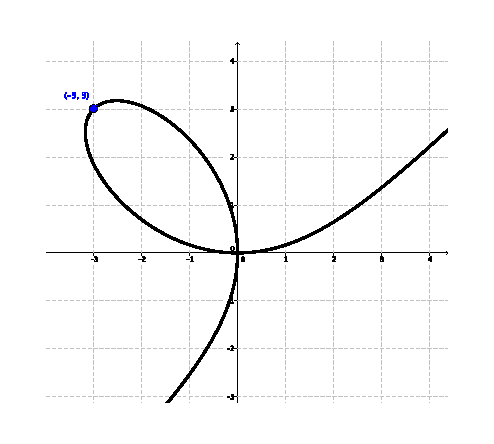
\includegraphics[width=0.5\textwidth]{a2-implicitplot2}
\end{center}

	\begin{parts}
		\part[10] Calculate a formula for $dy/dx$. Show all work.
		
		\vspace{2.5in}
		
		\part[4] Find an equation for the line tangent to the curve at $(-3,3)$. Show all your work and do not merely estimate values from the graph. 
		
		\vspace{2in}
		
		\part (BONUS CREDIT) From the graph you can see that there are two places where the tangent line to the curve is horizontal: at the origin, and at a point in the second quadrant. Find the exact coordinates of the one in the second quadrant. Show all work and make no estimations. 
	\end{parts}
	
\pageturn

\question[10] Compute the exact value of the following limit, justifying your work completely with proper notation, and using calculus: 
\[ \lim_{x \to 0} \frac{\cos(3x) - 1 - 3x^2}{7x^2} \]
(Hint: The limit does actually exist.) 


\pageturn

\question[6] Your response to the last question on this Assessment is to be typed up in an email and submitted to me (talbertr@gvsu.edu) no later than \textbf{5pm on Saturday, October 19}. Once again I am  soliciting your honest feedback on how the course is going so far with an emphasis this time on areas you feel are strengths and areas to work on. Please include anything you feel would be helpful in improving the course moving forward. You won't be penalized if you don't like everything (or anything!) and I certainly value your constructive criticism. The questions to address are: 
\begin{itemize}
	\item What's one thing related to the class that you definitely feel that you are better at doing now than you were eight weeks ago? This can be something mathematical or something more general like overall study habits. 
	\item Moving forward into the second half of the semester, what's one thing you feel you need to work on the most? Again this can be something mathematical or something more general. 
	\item Is there anything you'd like to mention at this time about the ``flipped'' setup of MTH 201 (where we have the lectures outside of class and do active work during class)? Among the things you might comment on are ways the flipped class is helping you learn, ways we could continue to improve the class to make you learn more, and so on. 
	\item Anything else you want to mention? 
\end{itemize}

\end{questions}


\end{document}